\subsection{Tests Objekterkennung}
\label{sec_testObj}
Die Objekterkennung wurde auf drei Arten getestet. Für diese Arbeit ist eine verlässliche Erkennung auf Simulationsbildern wichtig. Aus diesem Grund beziehen sich die ersten Tests auf Simulationsbildern. Der dritte Test dient der Evaluation der genutzten Methode in Bezug auf Echtdaten.\\
Die erste Testreihe besteht aus Bildern, auf denen das Objekt gut zu sehen ist und nur leicht verdeckt ist. Außerdem werden die Bilder so gewählt, dass teilweise in einzelnen Segmenten kein Objekt zu sehen ist und dass das Objekt über in verschiedenen Segmenten unterschiedlich Orientiert sind.\\
In der zweiten Testreihe werden die gleichen Bilder künstlich verschlechtert, um Bewegungsunschärfe und Rauschen der Kamera zu simulieren und die Grenzen der Objekterkennung im Bezug zur Bildqualität ermittelt. Für beide Testreihen wurden auch Vergleichsbilder ohne Objekt genommen.
\subsubsection*{Erste Testreihe}
\begin{figure}[H]
\begin{tabular}{cc}
\subfloat[]{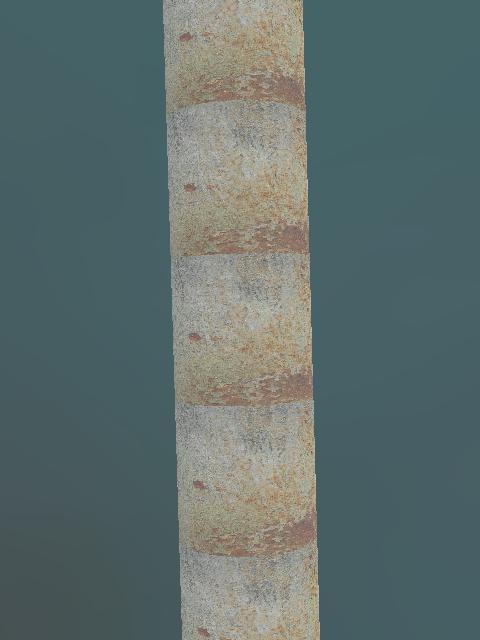
\includegraphics[scale=1]{/imageProcessing/gradeOptimal.jpg}}&
\subfloat[]{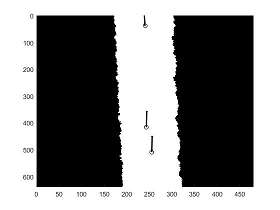
\includegraphics[scale=1]{/imageProcessing/gradeOptimalFin.jpg}}
\end{tabular}
\caption{Grades Objekt mit optimaler Qualität}
\end{figure}

\begin{figure}[H]
\begin{tabular}{cc}
\subfloat[]{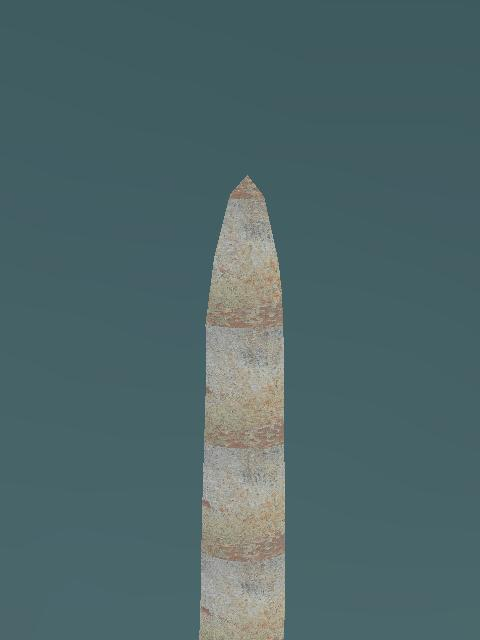
\includegraphics[scale=1]{/imageProcessing/gradeverborgen.jpg}}&
\subfloat[]{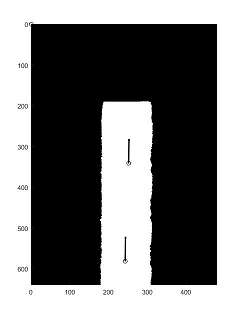
\includegraphics[scale=1]{/imageProcessing/gradeverborgenfin.jpg}}
\end{tabular}
\caption{Verdecktes Objekt mit optimaler Qualität}
\end{figure}

\begin{figure}[H]
\begin{tabular}{cc}
\subfloat[]{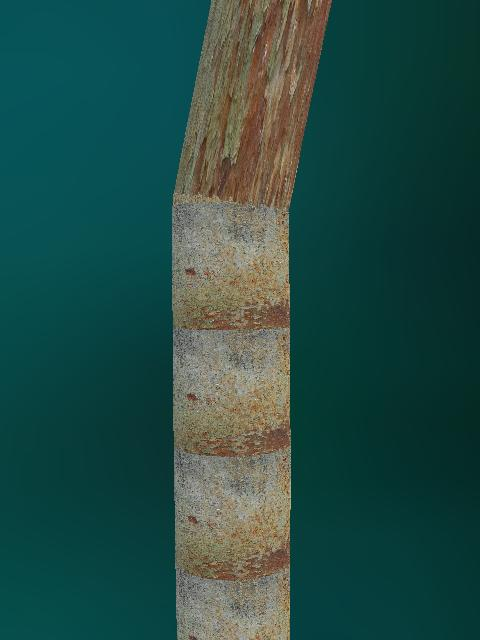
\includegraphics[scale=1]{/imageProcessing/knickOptimal.jpg}}&
\subfloat[]{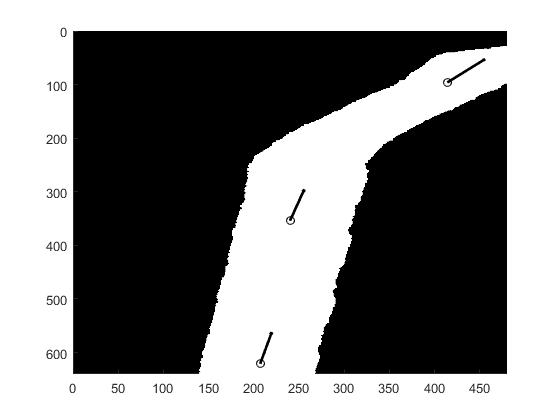
\includegraphics[scale=1]{/imageProcessing/knickoptimalfin.jpg}}
\end{tabular}
\caption{Geknicktes Objekt mit optimaler Qualität}
\end{figure}

\begin{figure}[H]
\begin{tabular}{cc}
\subfloat[]{
\includegraphics[scale=1]{/imageProcessing/nichts.jpg}}&
\subfloat[]{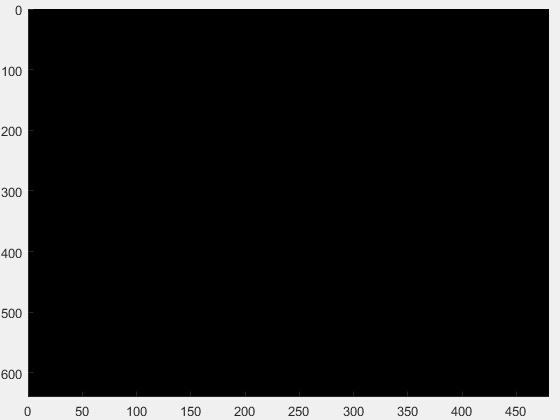
\includegraphics[scale=1]{/imageProcessing/nichtsoptimalfin.jpg}}
\end{tabular}
\caption{Kein Objekt mit optimaler Qualität}
\end{figure}

\subsubsection*{Zweite Testreihe}
\begin{figure}[H]
\begin{tabular}{cc}
\subfloat[]{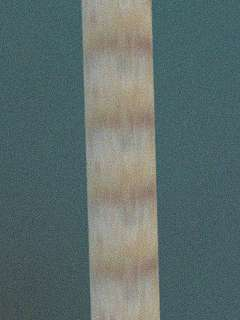
\includegraphics[scale=1]{/imageProcessing/graeOk.jpg}}&
\subfloat[]{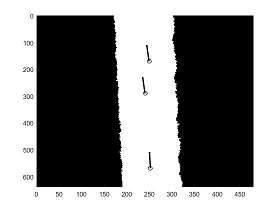
\includegraphics[scale=1]{/imageProcessing/graeOkFin.jpg}}
\end{tabular}
\caption{Grades Objekt mit verschlechterter Qualität}
\end{figure}

\begin{figure}[H]
\begin{tabular}{cc}
\subfloat[]{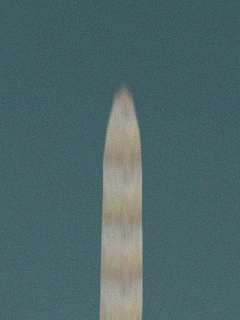
\includegraphics[scale=1]{/imageProcessing/gradeverborgenok.jpg}}&
\subfloat[]{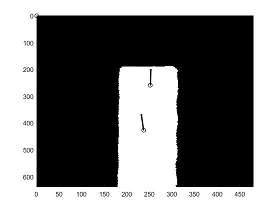
\includegraphics[scale=1]{/imageProcessing/gradeverborgenokfin.jpg}}
\end{tabular}
\caption{Verdecktes Objekt mit verschlechterter Qualität}
\end{figure}

\begin{figure}[H]
\begin{tabular}{cc}
\subfloat[]{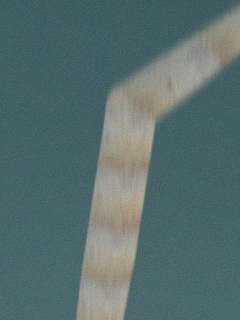
\includegraphics[scale=1]{/imageProcessing/knickok.jpg}}&
\subfloat[]{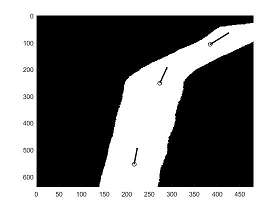
\includegraphics[scale=1]{/imageProcessing/knickokfin.jpg}}
\end{tabular}
\caption{Geknicktes Objekt mit verschlechterter Qualität}
\end{figure}

\begin{figure}[H]
\begin{tabular}{cc}
\subfloat[]{
\includegraphics[scale=1]{/imageProcessing/nichtsok.jpg}}&
\subfloat[]{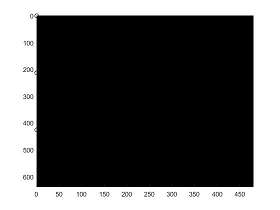
\includegraphics[scale=1]{/imageProcessing/nichtsokfin.jpg}}
\end{tabular}
\caption{Kein Objekt mit verschlechterter Qualität}
\end{figure}


\begin{figure}[H]
\begin{tabular}{cc}
\subfloat[]{
\includegraphics[scale=1]{/imageProcessing/gradeschlecht.jpg}}&
\subfloat[]{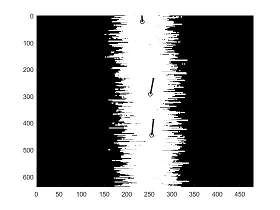
\includegraphics[scale=1]{/imageProcessing/gradeschlechtFin.jpg}}
\end{tabular}
\caption{Grades Objekt mit sehr schlechter Qualität}
\end{figure}

\begin{figure}[H]
\begin{tabular}{cc}
\subfloat[]{
\includegraphics[scale=1]{/imageProcessing/gradeverborgenschlecht.jpg}}&
\subfloat[]{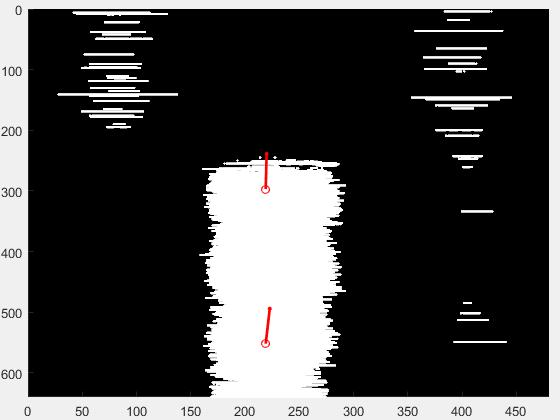
\includegraphics[scale=1]{/imageProcessing/gradeverborgenschlechtfin.jpg}}
\end{tabular}
\caption{Verdecktes Objekt mit sehr schlechter Qualität}
\end{figure}

\begin{figure}[H]
\begin{tabular}{cc}
\subfloat[]{
\includegraphics[scale=1]{/imageProcessing/knickschlecht.jpg}}&
\subfloat[]{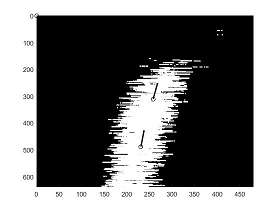
\includegraphics[scale=1]{/imageProcessing/knickschlechtfin.jpg}}
\end{tabular}
\caption{Geknicktes Objekt mit sehr schlechter Qualität}
\end{figure}

\begin{figure}[H]
\begin{tabular}{cc}
\subfloat[]{
\includegraphics[scale=1]{/imageProcessing/nichtsschlecht.jpg}}&
\subfloat[]{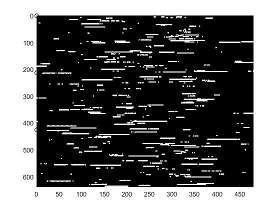
\includegraphics[scale=1]{/imageProcessing/nichtsschlechtfin.jpg}}
\end{tabular}
\caption{Kein Objekt mit sehr schlechter Qualität}
\end{figure}

\subsubsection*{Dritte Testreihe}
Um zu zeigen, dass das Verfahren auch bei echten Bildern funktioniert wurden insgesamt 12 Bilder [\ref{anhang_objdecttests}] aus einem Testlauf des AUVs \textit{DAGON}\footnote{http://robotik.dfki-bremen.de/de/forschung/robotersysteme/dagon.html} während des Projektes \textit{CUSLAM}\footnote{http://robotik.dfki-bremen.de/de/forschung/projekte/cuslam.html} im Unisee getestet. In einige Bilder, wie [\ref{rp_a}] oder [\ref{rp_b}] ist die Pipeline schwer zu erkennen. Dadurch muss der Schwellwert für das Template entsprechend niedrig gesetzt werden, was in vielen Punkten im Binärbild führt, die nicht zum Objekt gehören. In Bildern, in denen die Pipeline direkt angestrahlt wird und klar heller ist, wie in [\ref{rp_g}] oder [\ref{rp_j}] ist das Objekt wieder klar heller als der Hintergrund, der Schwellwert kann höher angesetzt werden und die Erkennung hat weniger Punkte im Binärbild.
%\begin{figure}[H]
%\begin{tabular}{ccc}
%\subfloat[]{\includegraphics[height=0.2\textheight,width=0.33\textwidth]{imageProcessing/1orgImstart.png}\label{rp_a}}&
%\subfloat[]{\includegraphics[height=0.2\textheight,width=0.33\textwidth]{imageProcessing/2orgImstart.png}\label{rp_b}}&
%\subfloat[]{\includegraphics[height=0.2\textheight,width=0.33\textwidth]{imageProcessing/3orgImstart.png}}\\
%\subfloat[]{\includegraphics[height=0.2\textheight,width=0.33\textwidth]{imageProcessing/4orgImstart.png}}&
%\subfloat[]{\includegraphics[height=0.2\textheight,width=0.33\textwidth]{imageProcessing/5orgImstart.png}}&
%\subfloat[]{\includegraphics[height=0.2\textheight,width=0.33\textwidth]{imageProcessing/6orgImstart.png}}\\
%\subfloat[]{\includegraphics[height=0.2\textheight,width=0.33\textwidth]{imageProcessing/7orgImstart.png}\label{rp_g}}&
%\subfloat[]{\includegraphics[height=0.2\textheight,width=0.33\textwidth]{imageProcessing/8orgImstart.png}}&
%\subfloat[]{\includegraphics[height=0.2\textheight,width=0.33\textwidth]{imageProcessing/9orgImstart.png}}\\
%\subfloat[]{\includegraphics[height=0.2\textheight,width=0.33\textwidth]{imageProcessing/10orgImstart.png}\label{rp_j}}&
%\subfloat[]{\includegraphics[height=0.2\textheight,width=0.33\textwidth]{imageProcessing/11orgImstart.png}}&
%\subfloat[]{\includegraphics[height=0.2\textheight,width=0.33\textwidth]{imageProcessing/12orgImstart.png}}
%\end{tabular}
%\caption{Pipeline Testbilder aufgenommen im Unisee vom AUV \textit{DAGON}. }
%\label{realData_all}
%\end{figure}